\documentclass[11pt]{article}
\usepackage{graphicx}
\usepackage{float}
\graphicspath{ {images/} }
\begin{document}

\begin{titlepage}

\begin{center}
\begin{huge}
Swarm Visualiser - COS 301 Main Project
\\
Functional Specification
\begin{small}
\\
Team: Dragon Brain
\\
Members:
\\
Matheu Botha u14284104
\\
Renton McInytre u14312710
\\
Emilio Singh u14006512
\\
Gerard van Wyk u14101263

\end{small}

\end{huge}
\end{center}
\end{titlepage}

\pagebreak

\tableofcontents

\pagebreak
\section{System Domain Model}
\paragraph{•}
In this section we will discuss and present a system-wide domain model and present the constituent systems, Modules, and their scopes

\begin{figure}[h]

\end{figure}
\section{Modules}
\subsection{General Optimiser}
\paragraph{•}
The General Optimiser or OPT for short is the module that provides the problem solving capacities of the system. It makes use of swarm-based methods to traverse user defined search spaces and perform evaluations of particles within the search space against user defined objective functions.
\subsubsection{Scope}
\paragraph{•}
The scope of the General Optimiser is presented below.
\begin{figure}[H]
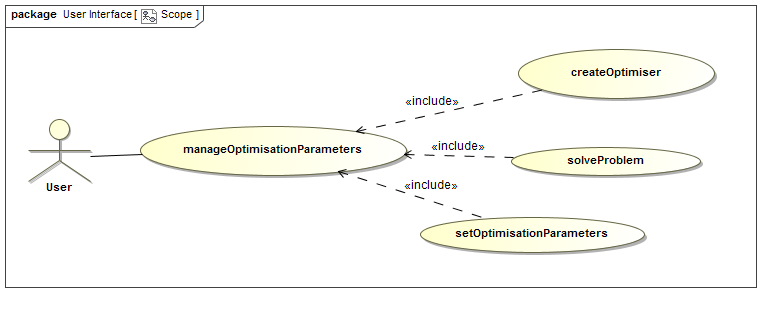
\includegraphics[scale=0.45]{Scope.png}
\end{figure}

\paragraph{•}
The User has 3 areas of general purpose use
\begin{itemize}
\item Creating Settings Packages which configure the Optimiser for runs
\item Changing Optimiser parameters during a run
\item Presenting problems for the Optimiser to solve
\end{itemize}
\subsubsection{Service Contracts}
\paragraph{•}
We will now specify the service contracts that importantly define the capacities of the General Optimiser Module

\subsubsection{Create Optimiser}
\begin{figure}[H]
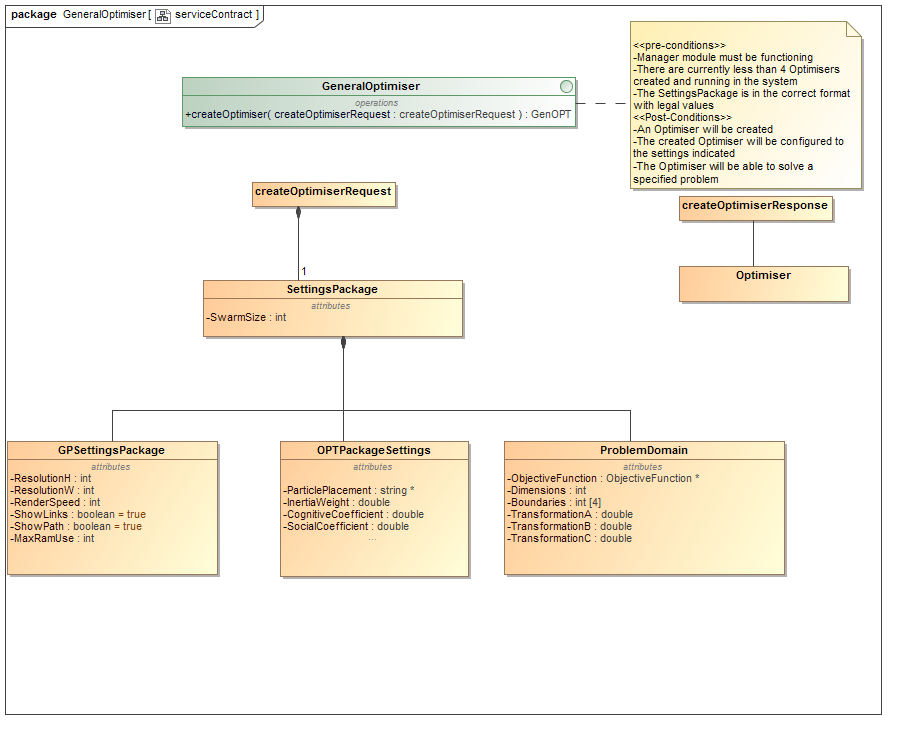
\includegraphics[scale=0.4]{serviceContractOPT.png}
\end{figure}

\paragraph{•}
The user will request for an Optimiser to be created. If there is space, that is less than 4 Optimisers already exist in the System, then the user will construct, indirectly, a SettingsPackage by entering their configuration parameters for the Optimiser. This Settings Package will be used by the Manager to construct and configure an Optimiser for use.

The exact conditions will be codified below:
\begin{enumerate}
\item There must be fewer than 4 Optimisers currently running in the system
\item The SettingsPackage received must contain specifications for all configuration parameters and must contain values for those parameters within legal domains.
\item The Manager Module is ready to receive/able to receive a new order/request from the User Interface.
\end{enumerate}

\subsubsection{Functional Requirements}
\begin{figure}[H]
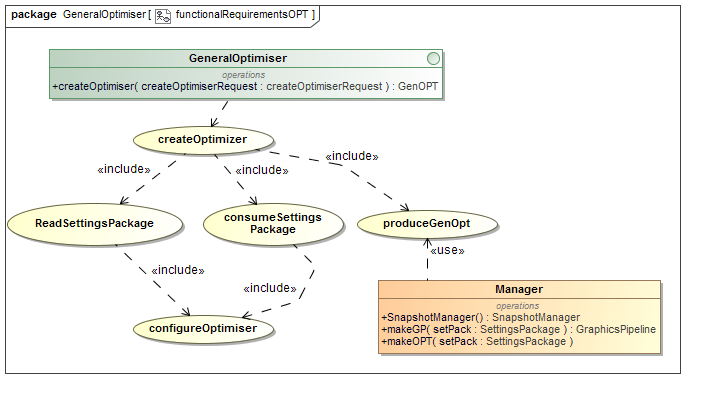
\includegraphics[scale=0.5]{functionalRequirementsOPT.png}
\end{figure}

\paragraph{•}
In terms of the functional requirements for the creation of an Optimiser object, a number of factors need to be considered in order for this to realised. Firstly, the reading and consumption of a Settings Package object relates to the process of extracting the necessary information from the settings package, the GenOPT package components, in order to provide the information during a constructor call. During the process, the Settings Package received is now invalidated and must be destroyed as it is at the end of its life-cycle. Once configuration has been completed, the GenOpt object will be produced and used by the Manager object.
\subsubsection{Process Design}
\paragraph{•}
The process specification defined here is for the process to create an Optimiser object.
\begin{figure}[H]
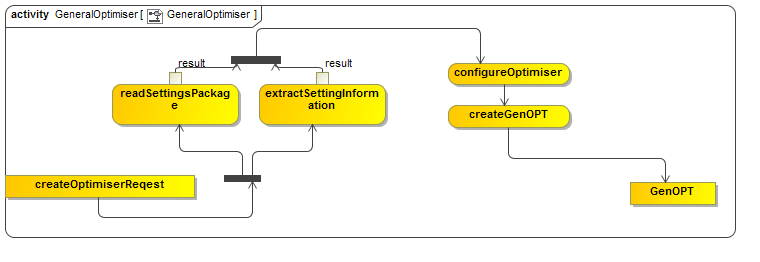
\includegraphics[scale=0.5]{GeneralOptimiserActivity.png}
\end{figure}

\subsubsection{Domain Model}
\paragraph{•}
Presented below is the domain model of the General Optimiser.
\begin{figure}[H]
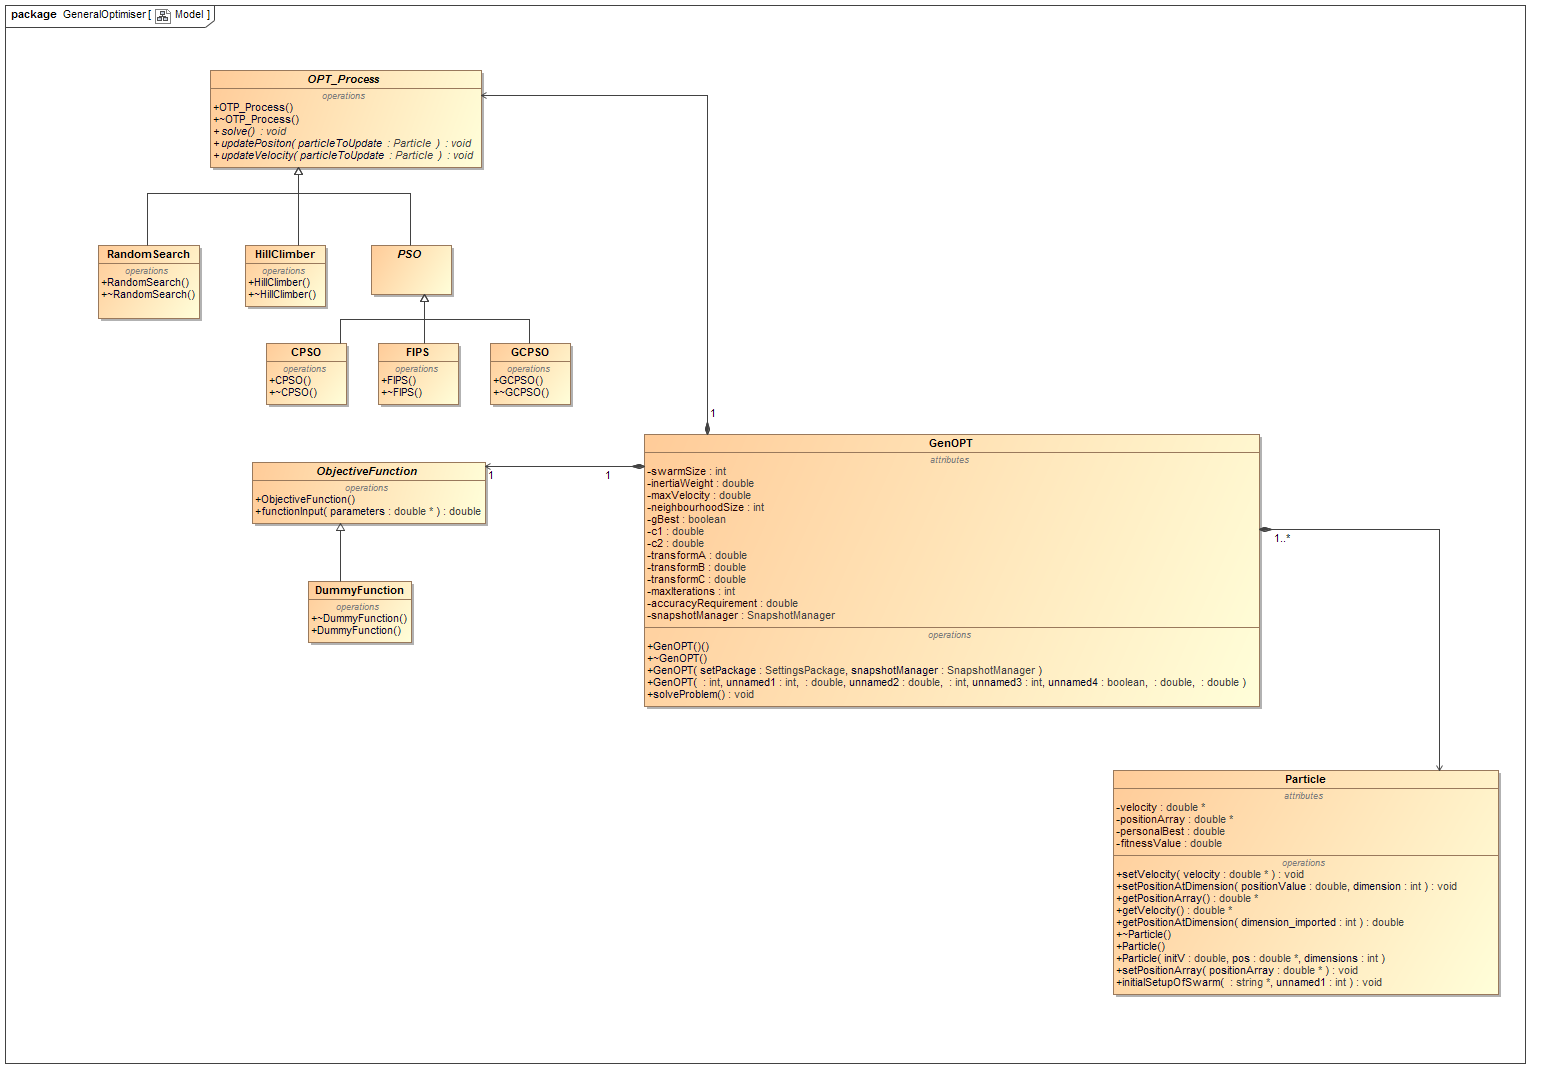
\includegraphics[scale=0.2]{OPTModel.png}
\end{figure}

\subsection{Graphics Processor}
The Graphics Processor is responsible for visualising the data that is generated by the Optimiser. 

\subsubsection{Scope}
The scope for the Graphics Processor is presented below:
\begin{figure}[H]
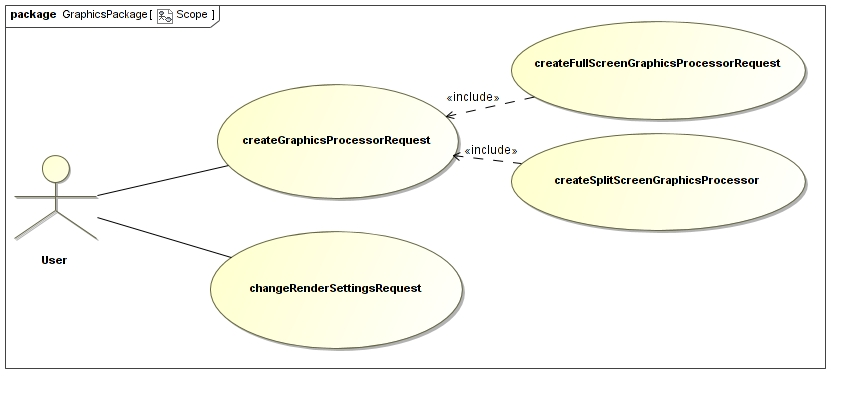
\includegraphics[scale=0.45]{GraphicsProcessor/Scope.jpg}
\end{figure} 
\paragraph{•}
The User has 2 areas of general purpose use
\begin{itemize}
\item Creating a Graphics processor to visualize a swarm which can be done in to ways:
\begin{itemize}
\item Full screen mode for a single swarm visualiser.
\item Split screen mode for multiple swarms.
\end{itemize}
\item Change the render settings
\end{itemize}

\subsubsection{Service Contracts}
\begin{figure}[H]
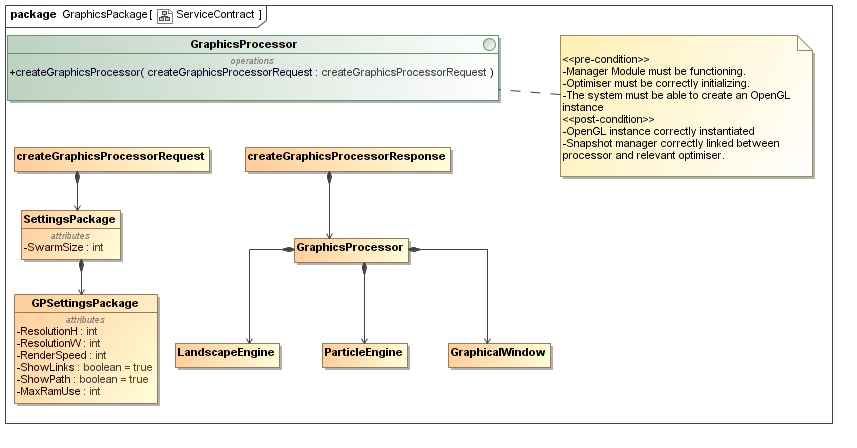
\includegraphics[scale=0.45]{GraphicsProcessor/ServiceContract.jpg}
\end{figure}
The service contract for the graphics processor facilitates the creation of the processor. A graphics processor as a whole is a single entity which can then be associated with a optimiser. Once associated with that optimiser in the manager, the data from the optimiser will be visualised. 

\subsubsection{Functional Requirements}
\begin{figure}[H]
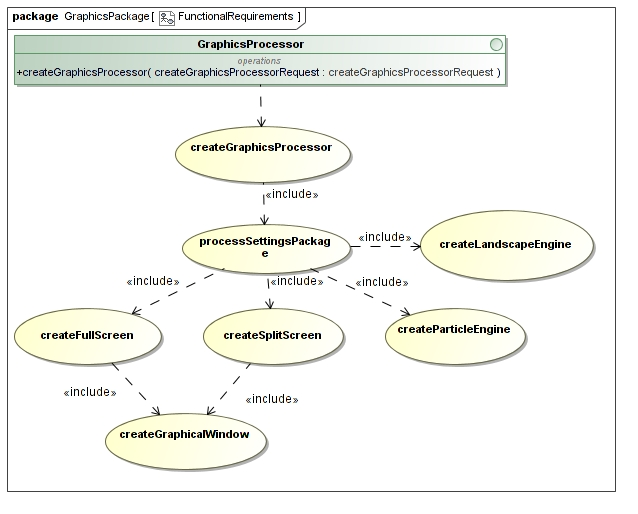
\includegraphics[scale=0.45]{GraphicsProcessor/FunctionalRequirements.jpg}
\end{figure}
The functional requirements for creating a graphics processor are defined as follows:
It will recieve a settings package. Determine how many optimizers will be running which will inform it whether or not it needs a split screen functionality. And then simply pass the render settings to the shaders.

\subsubsection{Process Design}
The following is the process design for creating a graphical processor:
\begin{figure}[H]
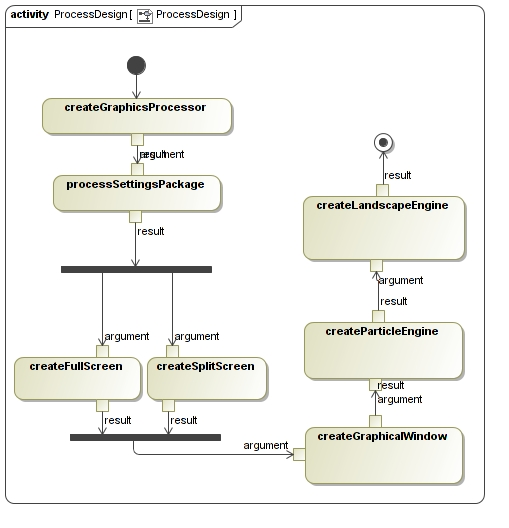
\includegraphics[scale=0.45]{GraphicsProcessor/ProcessDesign.jpg}
\end{figure}

\subsubsection{DomainModel}
\begin{figure}[H]
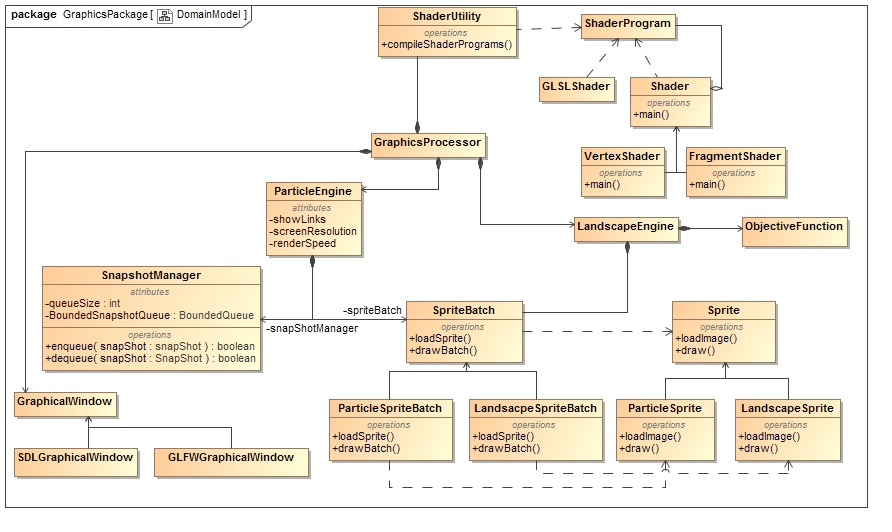
\includegraphics[scale=0.45]{GraphicsProcessor/DomainModel.jpg}
\end{figure}

\subsection{Manager}
\subsubsection{Scope}
\begin{figure}[H]
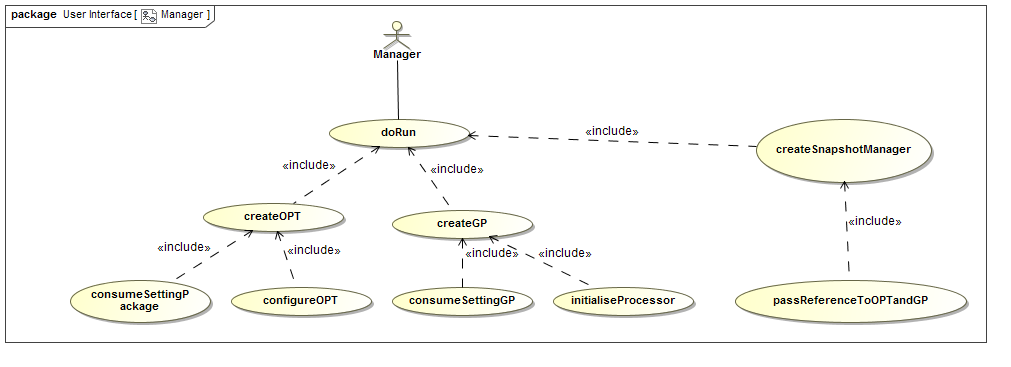
\includegraphics[scale=0.45]{Manager.png}
\end{figure}
\paragraph{•}
The scope of the Manager model can be defined in the context of a single doRun operation. A run is defined as the interaction between an optimiser and a graphics process mediated by the snapshot manager serving as the intermediate storage unit. The doRun operation will create the requisite components who will then in turn perform their operation once notified by their partners in the communication.

\subsubsection{Domain Model}
\begin{figure}[H]
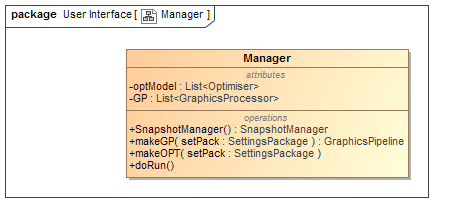
\includegraphics[scale=0.45]{ManagerModel.png}
\end{figure}
\paragraph{•}
The Manager class encapsulates the core functioning integration unit of the system. The Manager class will contain references to specific Optimisers and Graphics Processors and Snapshot Managers. One set of the three components comprises the components needed to perform a run. Each of these components are tethered, or coupled, to each other for the duration of the run and cannot be uncoupled. This will end when the run is terminated with the components being destroyed and the resources allocated available for reuse after the fact.
\subsection{User Interface}
\subsubsection{Scope}
The scope of the User Interface is presented below.
\begin{figure}[H]
	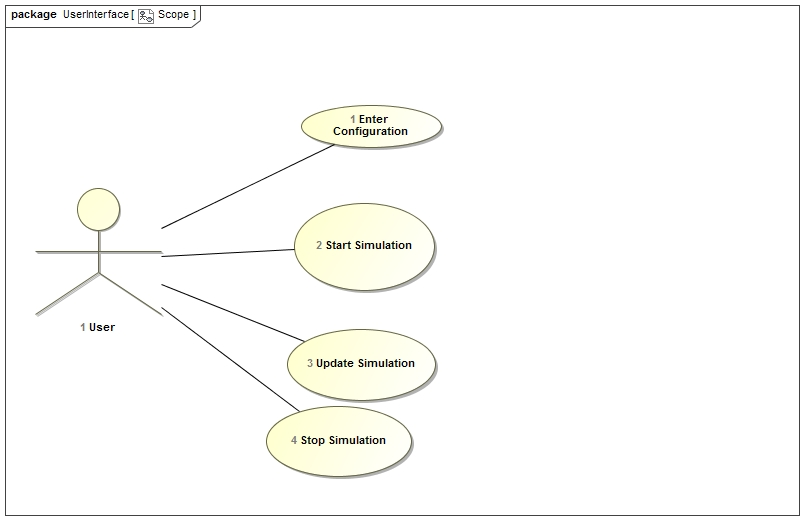
\includegraphics[scale=0.45]{GUI_Scope.jpg}
\end{figure}

\paragraph{•}
The User has 4 main capabilities
\begin{itemize}
	\item Changing the parameters of run environment
	\item Starting the simulation with the currently configured parameters.
	\item Updating the parameters of the current simulation based on the current (newly configured) parameters.
	\item Stopping the current simulation.
\end{itemize}

\subsubsection{Functional Requirements}
In terms of the Functional Requirements of the User Interface, the focus is as follows:
\begin{itemize}
	\item The user must be able to configure parameters for the system via the GUI.
	\item The GUI should be capable of sending data to the SettingsPackage in order to generate a SettingsPackage.
	\item The system should generate a SettingsPackage and start the simulation upon user request.
	\item The user should be able to edit configuration mid-run
\end{itemize}

\subsubsection{Activity Diagram}
Following is an activity diagram for the process involved in starting a run of the project.
\begin{figure}[H]
	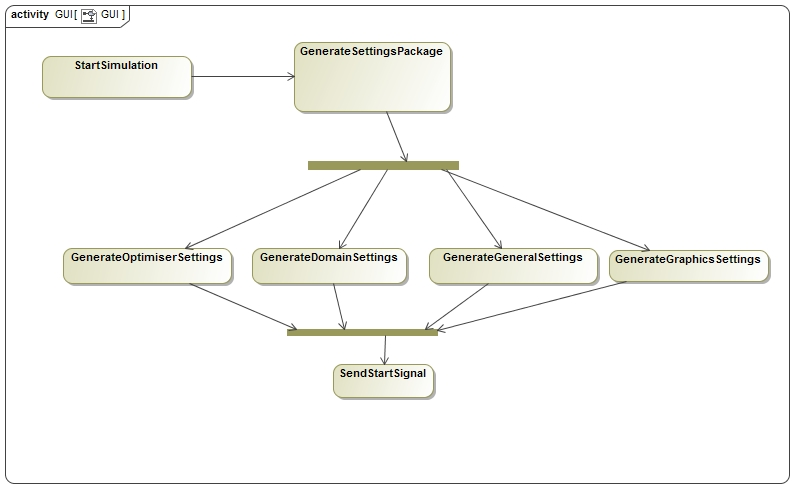
\includegraphics[scale=0.45]{GUI_Activity.jpg}
\end{figure}

\section{System Use Cases}
\subsection{System Usage}
\subsubsection{In-Run}
\paragraph{•}
The following use case diagram highlights the user actions during the system operation
\begin{figure}[H]
	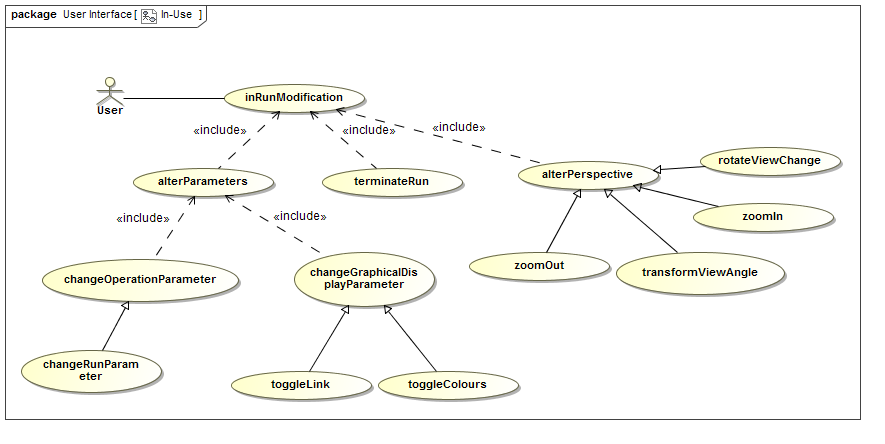
\includegraphics[scale=0.55]{inUse.png}
\end{figure}

\section{Algorithm Service Contracts}
\paragraph{•}
This project relies very heavily on its algorithms and their complexity is amongst the most difficult to implement and difficult to understand components of the project as a whole. Therefore, this section will deal with explaining how each of the algorithms and their components function as well codify the behaviour, functioning and operation of the algorithms in use in the system. 
\subsection{Algorithms}
\subsubsection{Operations and Limitations}
\paragraph{•}
To clarify, we will define some terms below
\begin{itemize}
\item Swarm- A collection of particles that is used to solve an optimisation problem
\item Particle- A single worker unit of the Swarm that contains a position reference and solution variables to the problem being solved.
\item Run - A run refers to a single span of time that starts when an optimiser is configured by the user and started. The run ends when the user decides to terminate the visualisation or the stopping conditions of the optimiser bring it to an end.
\item Iteration - An iteration is a single unit of work for an optimiser. An iteration consists of updating all of the particles in the swarm in terms of their positions and velocities and determining if an ideal solution has been worked out yet.
\item Optimiser - A Swarm based manager component that contains a swarm, a problem and will then make use of iterations in order to produce solutions to the given problem
\item Velocity - A rate of change used by the particle to quantify how far per iteration it is able to move. This can change and is influenced by many factors like other particles or previous histories.
\item Position - A set of parameters that indicate where in the problem domain the particle is in terms of mapping a given set of parameters to a given result in the problem space based on the function given.
\item Stopping Conditions- These are specific conditions with regards to system parameters that when reached, are used to terminate an optimiser's functioning and stop it from continuing indefinitely. Examples include
\begin{itemize}
\item Maximum Iterations Reached
\item Sufficient solution accuracy reached
\item Insufficient change of particle positions
\item Approximate solution found
\item Premature Halt signalled by operator
\end{itemize}

\end{itemize}


\paragraph{•}
Specific Functioning Limitations 
\\
The project offers functionality in terms of user interaction in two areas
\begin{verbatim}
1) Configuring an Optimiser Run

	1. The system functioning takes place in terms of the user using the GUI to configure the initial settings for an optimiser.
	2. Once configured, the user will then start the run which will begin the optimisation process.

		1. The user can create and have up to 4 simultaneous runs at a given time depending on their hardware capacities and screen size.

2) Viewing and Changing the Visualisation

	1. Once the user has started the visualisation process, they can perform the following actions
		1. Change specific optimiser parameters that will take effect either
			1. During the next run: these will be configuration parameters such as Cognitive Coefficient
			2. In real time: these will be visualisation parameters such as viewing links

		2. Change viewing angle -This will happen by rotating the viewing plane or shifting the camera perspective focus

		3. Stop the run and terminate the optimiser in progress

There are some limitations to what the SwarmViz project can do.

1. It can only visualise 2D and 1D problems those being problems with 1 or 2 dimensions or input variables. 
2. It cannot in real time change the function being used
3. Arbitrary functions cannot be inserted into the system during run time. New functions will have to be programmed into the system and the system recompiled. However the function framework is modular enough that new functions can be inserted into the system with minimal code changes/effects on the existing system.

\end{verbatim}

\paragraph{•}
In general, the algorithm for an Optimiser is presented below.

\begin{enumerate}
\item Start of Run
\item Initialise Particles in Swarm with:
	\begin{enumerate}
	\item Positions
		\begin{itemize}
		\item Random Positions within Domain
		\item Specified Positions by user

		\end{itemize}	 
	\item Velocities as per random distribution
		
	\end{enumerate}
	\item Evaluate particle fitness of each particle in Swarm
		\begin{enumerate}
		\item Fitness=fitnessFunctionEvaluation(Particle[x])
		\end{enumerate}
\item Find and update best history and global best
\item Calculate and update each particle's new velocity
\item Update position of all particles by new velocity  
\item	Are any stopping conditions satisfied?
	\begin{enumerate}
	\item If so, HALT
	\item Otherwise go back to 3
		\begin{enumerate}
		\item Output graphical updates to Snapshot Manager
		\end{enumerate}
	\end{enumerate}
	
\item Run Terminated	
\end{enumerate}

\paragraph{•}
This process is also represented in the following flowchart
\begin{figure}[H]
	\includegraphics[scale=0.45]{flowchart.png}
\end{figure}

\paragraph{•}
This process is also represented in the following activity diagram
\begin{figure}[H]
	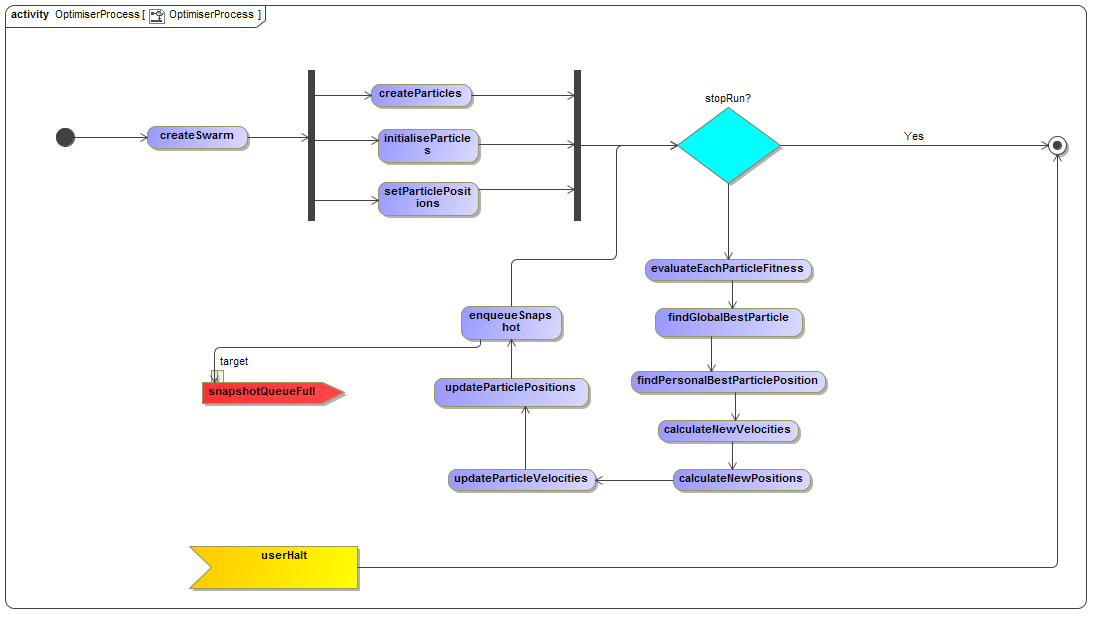
\includegraphics[scale=0.40]{OptimiserProcess.png}
\end{figure}

\end{document}
